\documentclass[tikz,border=10pt]{standalone}
% Shared look for every TikZ diagram. Load with % Shared look for every TikZ diagram. Load with % Shared look for every TikZ diagram. Load with \input{../../tools/tikz-style.tex}
\usepackage[T1]{fontenc}
\usepackage{lmodern}
\renewcommand{\sfdefault}{lmr}  % diagrams use the same serif as the text
\usetikzlibrary{arrows.meta, positioning, shapes.geometric, calc, fit, backgrounds}
\definecolor{cblue}{HTML}{4C78A8}
\definecolor{corange}{HTML}{F58518}
\definecolor{cgreen}{HTML}{54A24B}
\definecolor{cred}{HTML}{E45756}
\definecolor{cpurple}{HTML}{B279A2}
\definecolor{cgrey}{HTML}{6B6B6B}
\tikzset{
  every picture/.style={font=\sffamily, line width=1.2pt},
  box/.style={draw=#1, fill=#1!12, rounded corners=4pt, align=center, inner sep=7pt, minimum height=1.1cm},
  box/.default=cgrey,
  arrow/.style={-{Stealth[length=3mm]}, draw=cgrey, line width=1.4pt},
  title/.style={font=\sffamily\bfseries\Large},
  note/.style={font=\sffamily\small, text=cgrey, align=center},
}
\AtBeginDocument{\hyphenpenalty=10000 \exhyphenpenalty=10000}

\usepackage[T1]{fontenc}
\usepackage{lmodern}
\renewcommand{\sfdefault}{lmr}  % diagrams use the same serif as the text
\usetikzlibrary{arrows.meta, positioning, shapes.geometric, calc, fit, backgrounds}
\definecolor{cblue}{HTML}{4C78A8}
\definecolor{corange}{HTML}{F58518}
\definecolor{cgreen}{HTML}{54A24B}
\definecolor{cred}{HTML}{E45756}
\definecolor{cpurple}{HTML}{B279A2}
\definecolor{cgrey}{HTML}{6B6B6B}
\tikzset{
  every picture/.style={font=\sffamily, line width=1.2pt},
  box/.style={draw=#1, fill=#1!12, rounded corners=4pt, align=center, inner sep=7pt, minimum height=1.1cm},
  box/.default=cgrey,
  arrow/.style={-{Stealth[length=3mm]}, draw=cgrey, line width=1.4pt},
  title/.style={font=\sffamily\bfseries\Large},
  note/.style={font=\sffamily\small, text=cgrey, align=center},
}
\AtBeginDocument{\hyphenpenalty=10000 \exhyphenpenalty=10000}

\usepackage[T1]{fontenc}
\usepackage{lmodern}
\renewcommand{\sfdefault}{lmr}  % diagrams use the same serif as the text
\usetikzlibrary{arrows.meta, positioning, shapes.geometric, calc, fit, backgrounds}
\definecolor{cblue}{HTML}{4C78A8}
\definecolor{corange}{HTML}{F58518}
\definecolor{cgreen}{HTML}{54A24B}
\definecolor{cred}{HTML}{E45756}
\definecolor{cpurple}{HTML}{B279A2}
\definecolor{cgrey}{HTML}{6B6B6B}
\tikzset{
  every picture/.style={font=\sffamily, line width=1.2pt},
  box/.style={draw=#1, fill=#1!12, rounded corners=4pt, align=center, inner sep=7pt, minimum height=1.1cm},
  box/.default=cgrey,
  arrow/.style={-{Stealth[length=3mm]}, draw=cgrey, line width=1.4pt},
  title/.style={font=\sffamily\bfseries\Large},
  note/.style={font=\sffamily\small, text=cgrey, align=center},
}
\AtBeginDocument{\hyphenpenalty=10000 \exhyphenpenalty=10000}

\begin{document}
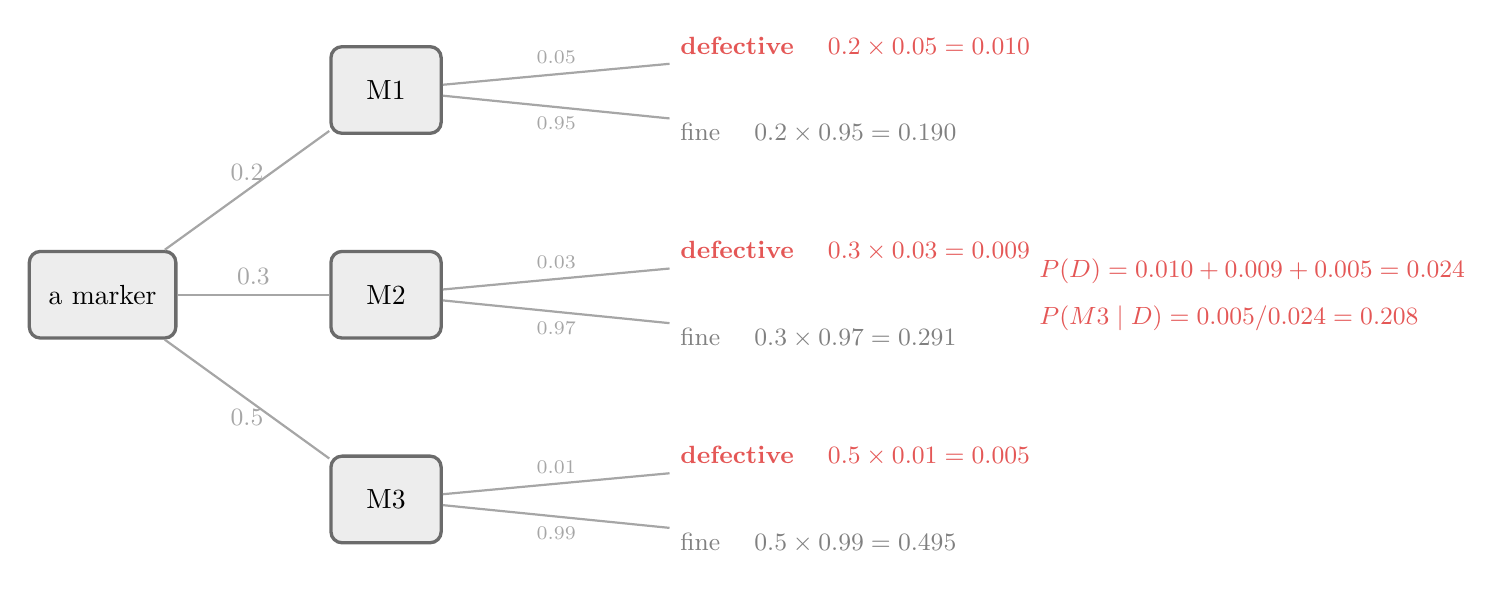
\begin{tikzpicture}[grow=right, level distance=3.6cm,
    level 1/.style={sibling distance=2.6cm}, level 2/.style={sibling distance=1.1cm},
    edge from parent/.style={draw, thick, gray!70},
    m/.style={box, minimum width=1.4cm}, leaf/.style={font=\small, anchor=west}]
  \node[box] {a marker}
    child {node[m] {M3}
      child {node[leaf, text=gray] {fine \quad $0.5 \times 0.99 = 0.495$} edge from parent node[below, font=\scriptsize] {0.99}}
      child {node[leaf, text=cred] {\textbf{defective} \quad $0.5 \times 0.01 = 0.005$} edge from parent node[above, font=\scriptsize] {0.01}}
      edge from parent node[below, font=\small] {0.5}}
    child {node[m] {M2}
      child {node[leaf, text=gray] {fine \quad $0.3 \times 0.97 = 0.291$} edge from parent node[below, font=\scriptsize] {0.97}}
      child {node[leaf, text=cred] {\textbf{defective} \quad $0.3 \times 0.03 = 0.009$} edge from parent node[above, font=\scriptsize] {0.03}}
      edge from parent node[above, font=\small] {0.3}}
    child {node[m] {M1}
      child {node[leaf, text=gray] {fine \quad $0.2 \times 0.95 = 0.190$} edge from parent node[below, font=\scriptsize] {0.95}}
      child {node[leaf, text=cred] {\textbf{defective} \quad $0.2 \times 0.05 = 0.010$} edge from parent node[above, font=\scriptsize] {0.05}}
      edge from parent node[above, font=\small] {0.2}};
  \node[align=left, text=cred, font=\small] at (14.6,0) {$P(D) = 0.010 + 0.009 + 0.005 = 0.024$\\[6pt] $P(M3 \mid D) = 0.005 / 0.024 = 0.208$};
\end{tikzpicture}
\end{document}
